% created on 25/11/2020
% @author : ebazan

\chapter{Color and Texture Retrieved Images: Some Cases of Study}\label{ch:suplementary_material_retrieval_systems}

\section{Color-based Image Retrieval}\label{sec:sm_color:class}
The figures \ref{fig:wonderwoman_distances} and \ref{fig:superman_distances} present the result of the classification of the images of two superhero toys. The query image is displayed in the upper left. The rows of the image arrangement represent the different measurements used in the retrieval while the columns show the most similar image from left to right in descending order. The numerical values of the distances are below each image; these values are not normalized nor are they on the same scale.

The two examples here show how, under certain disturbances in color distribution, bin-to-bin measurements are not able to identify the correct result. In the case of the wonderwoman toy, the fact that the query image has an extra accessory modifies the color signature of the figure, while in the case of the superman toy the color signature is very close to those toys that contain red and blue colors. These two images were obtained using the LAB color space and 32 bins for the pixels color distribution.
\begin{figure}[!ht]
 \centering    
 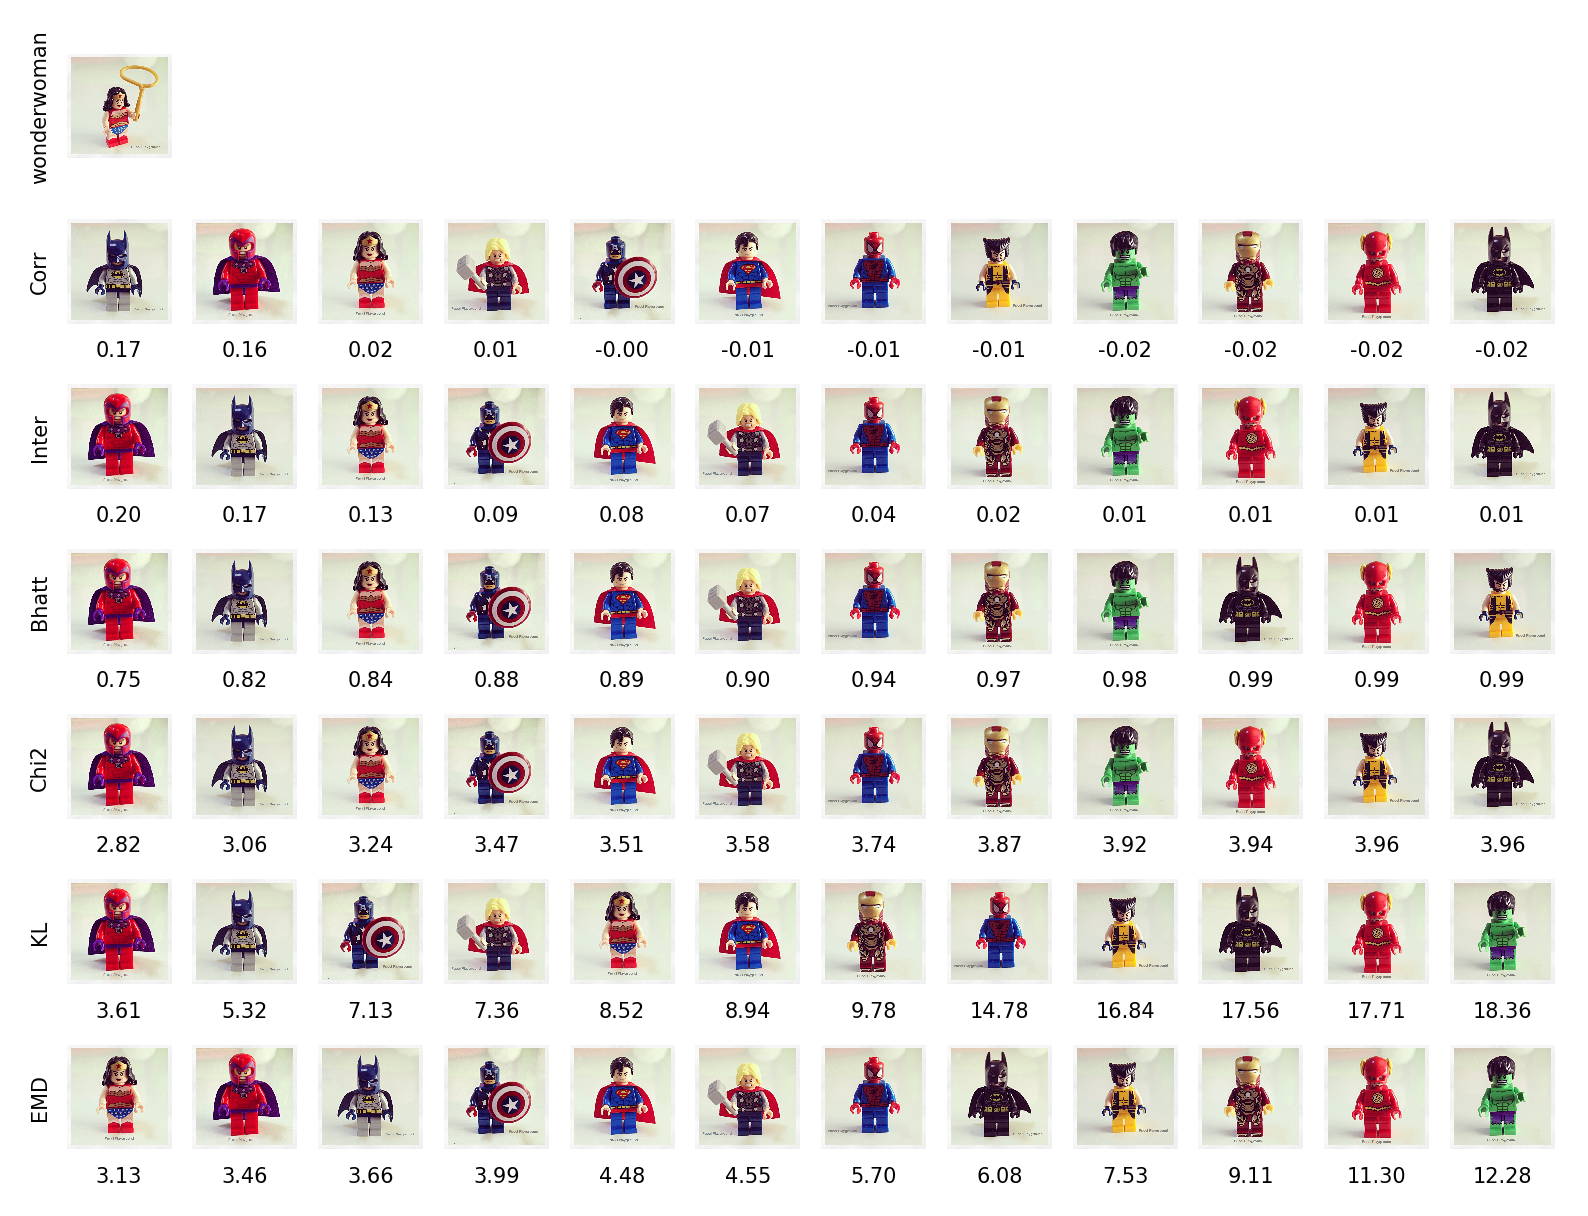
\includegraphics[width=0.9\textwidth]{cmpr_32_bins_lab_wonderwoman}
 \caption{Wonderwoman toy image retrieval example}
 \label{fig:wonderwoman_distances}
\end{figure}

\begin{figure}[!ht]
 \centering    
 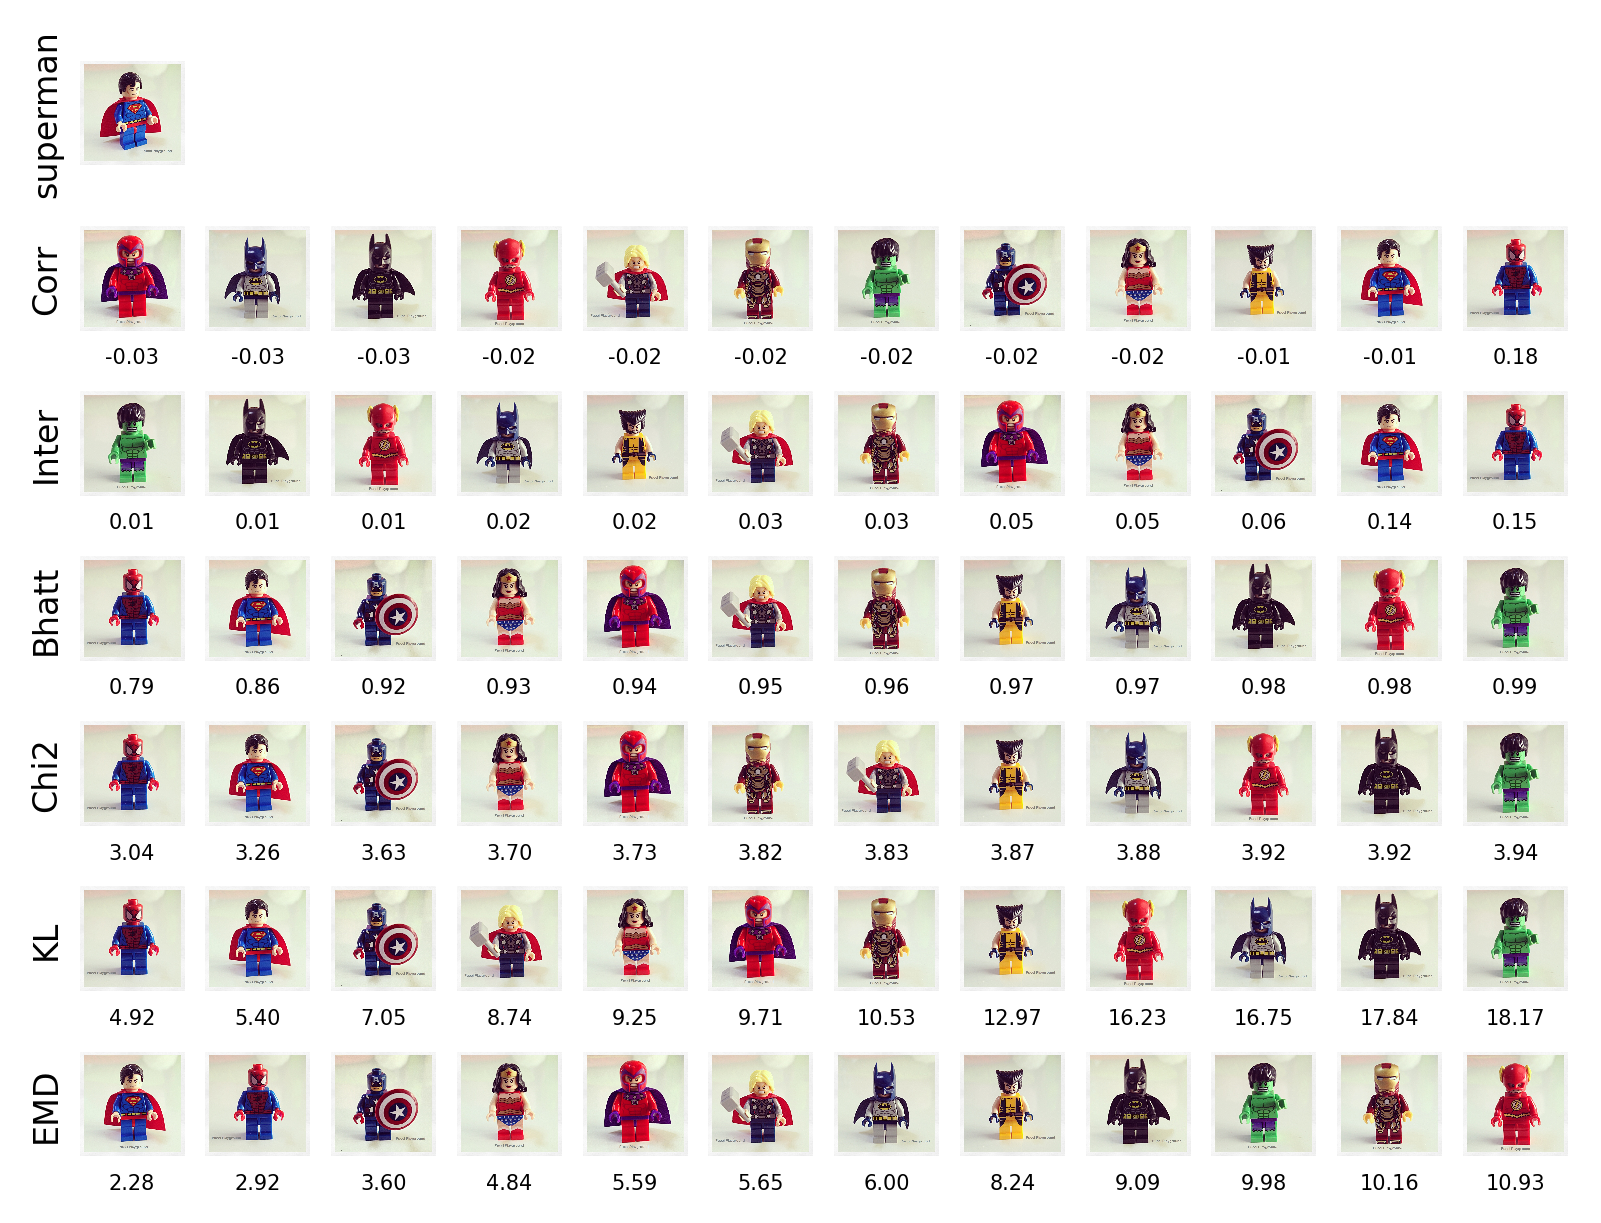
\includegraphics[width=0.9\textwidth]{cmpr_32_bins_lab_superman}
 \caption{Superman toy image retrieval example}
 \label{fig:superman_distances}
\end{figure}

\pagebreak
\section{Texture Projection Visual Evaluation}\label{sec:sm_mds}

The following images serve as a visual tool for the comparative evaluation of the different measures analyzed in the main article. As we described in section \ref{subsec:mds}, the MDS technique allows to projecting the textures in a low dimensional space using the distances given by the similarity measures. This representation is carried out in a two-dimensional Euclidean space in our case. In the figures, we can notice that the MDS technique has problems to represent coherently the textures when the input measures are not a metric, i.e., for the bin-to-bin measures. The axis in  Figs. \ref{fig:MDS_Inter} to \ref{fig:MDS_KL} do not correspond with the input space of the textures. 

However, in the case of EMD, we can observe that since this measure uses a ground distance to calculate the similarity, we can define the cost matrix $\mathbf{C}_{ij} = c(x_i, y_j)$ of Eq. \ref{eq:optimal_work} to be the $L_1$-distance as
\begin{eqnarray} 
 c(x_i, y_i) = d((\omega_i, \theta_i), (\omega_j, \theta_j))=\alpha|\Delta \omega| + |\Delta \theta| \label{eq:ground_distance}
\end{eqnarray}
where $|\Delta \omega| = \omega_i - \omega_j$, $\Delta \theta=min(|\theta_i-\theta_j|, \theta_{max} - |\theta_i-\theta_j|)$, and $\alpha$ is a constant that regulates the importence between the orientation and the coarsness of textures. In such a way that it represents the 2D texture distributions into a log-polar space. 
In the image \ref{fig:MDS_EMD}, we can distinguish this effect because the textures are organized concerning their orientation and frequency into a log-polar coordinate space forming a circle. The orientation of texture is represented along the circle while the frequency follows the axis that goes from the outside of the circle to the center, where the lower frequency images remain at the edge of the circle and those with high frequency (and low directionality) are grouped in the center. This behavior is not shown with any of the other measures and is reflected in the stress value of the figure~\ref{fig:stress}.

\begin{figure}[!ht]
 \centering    
 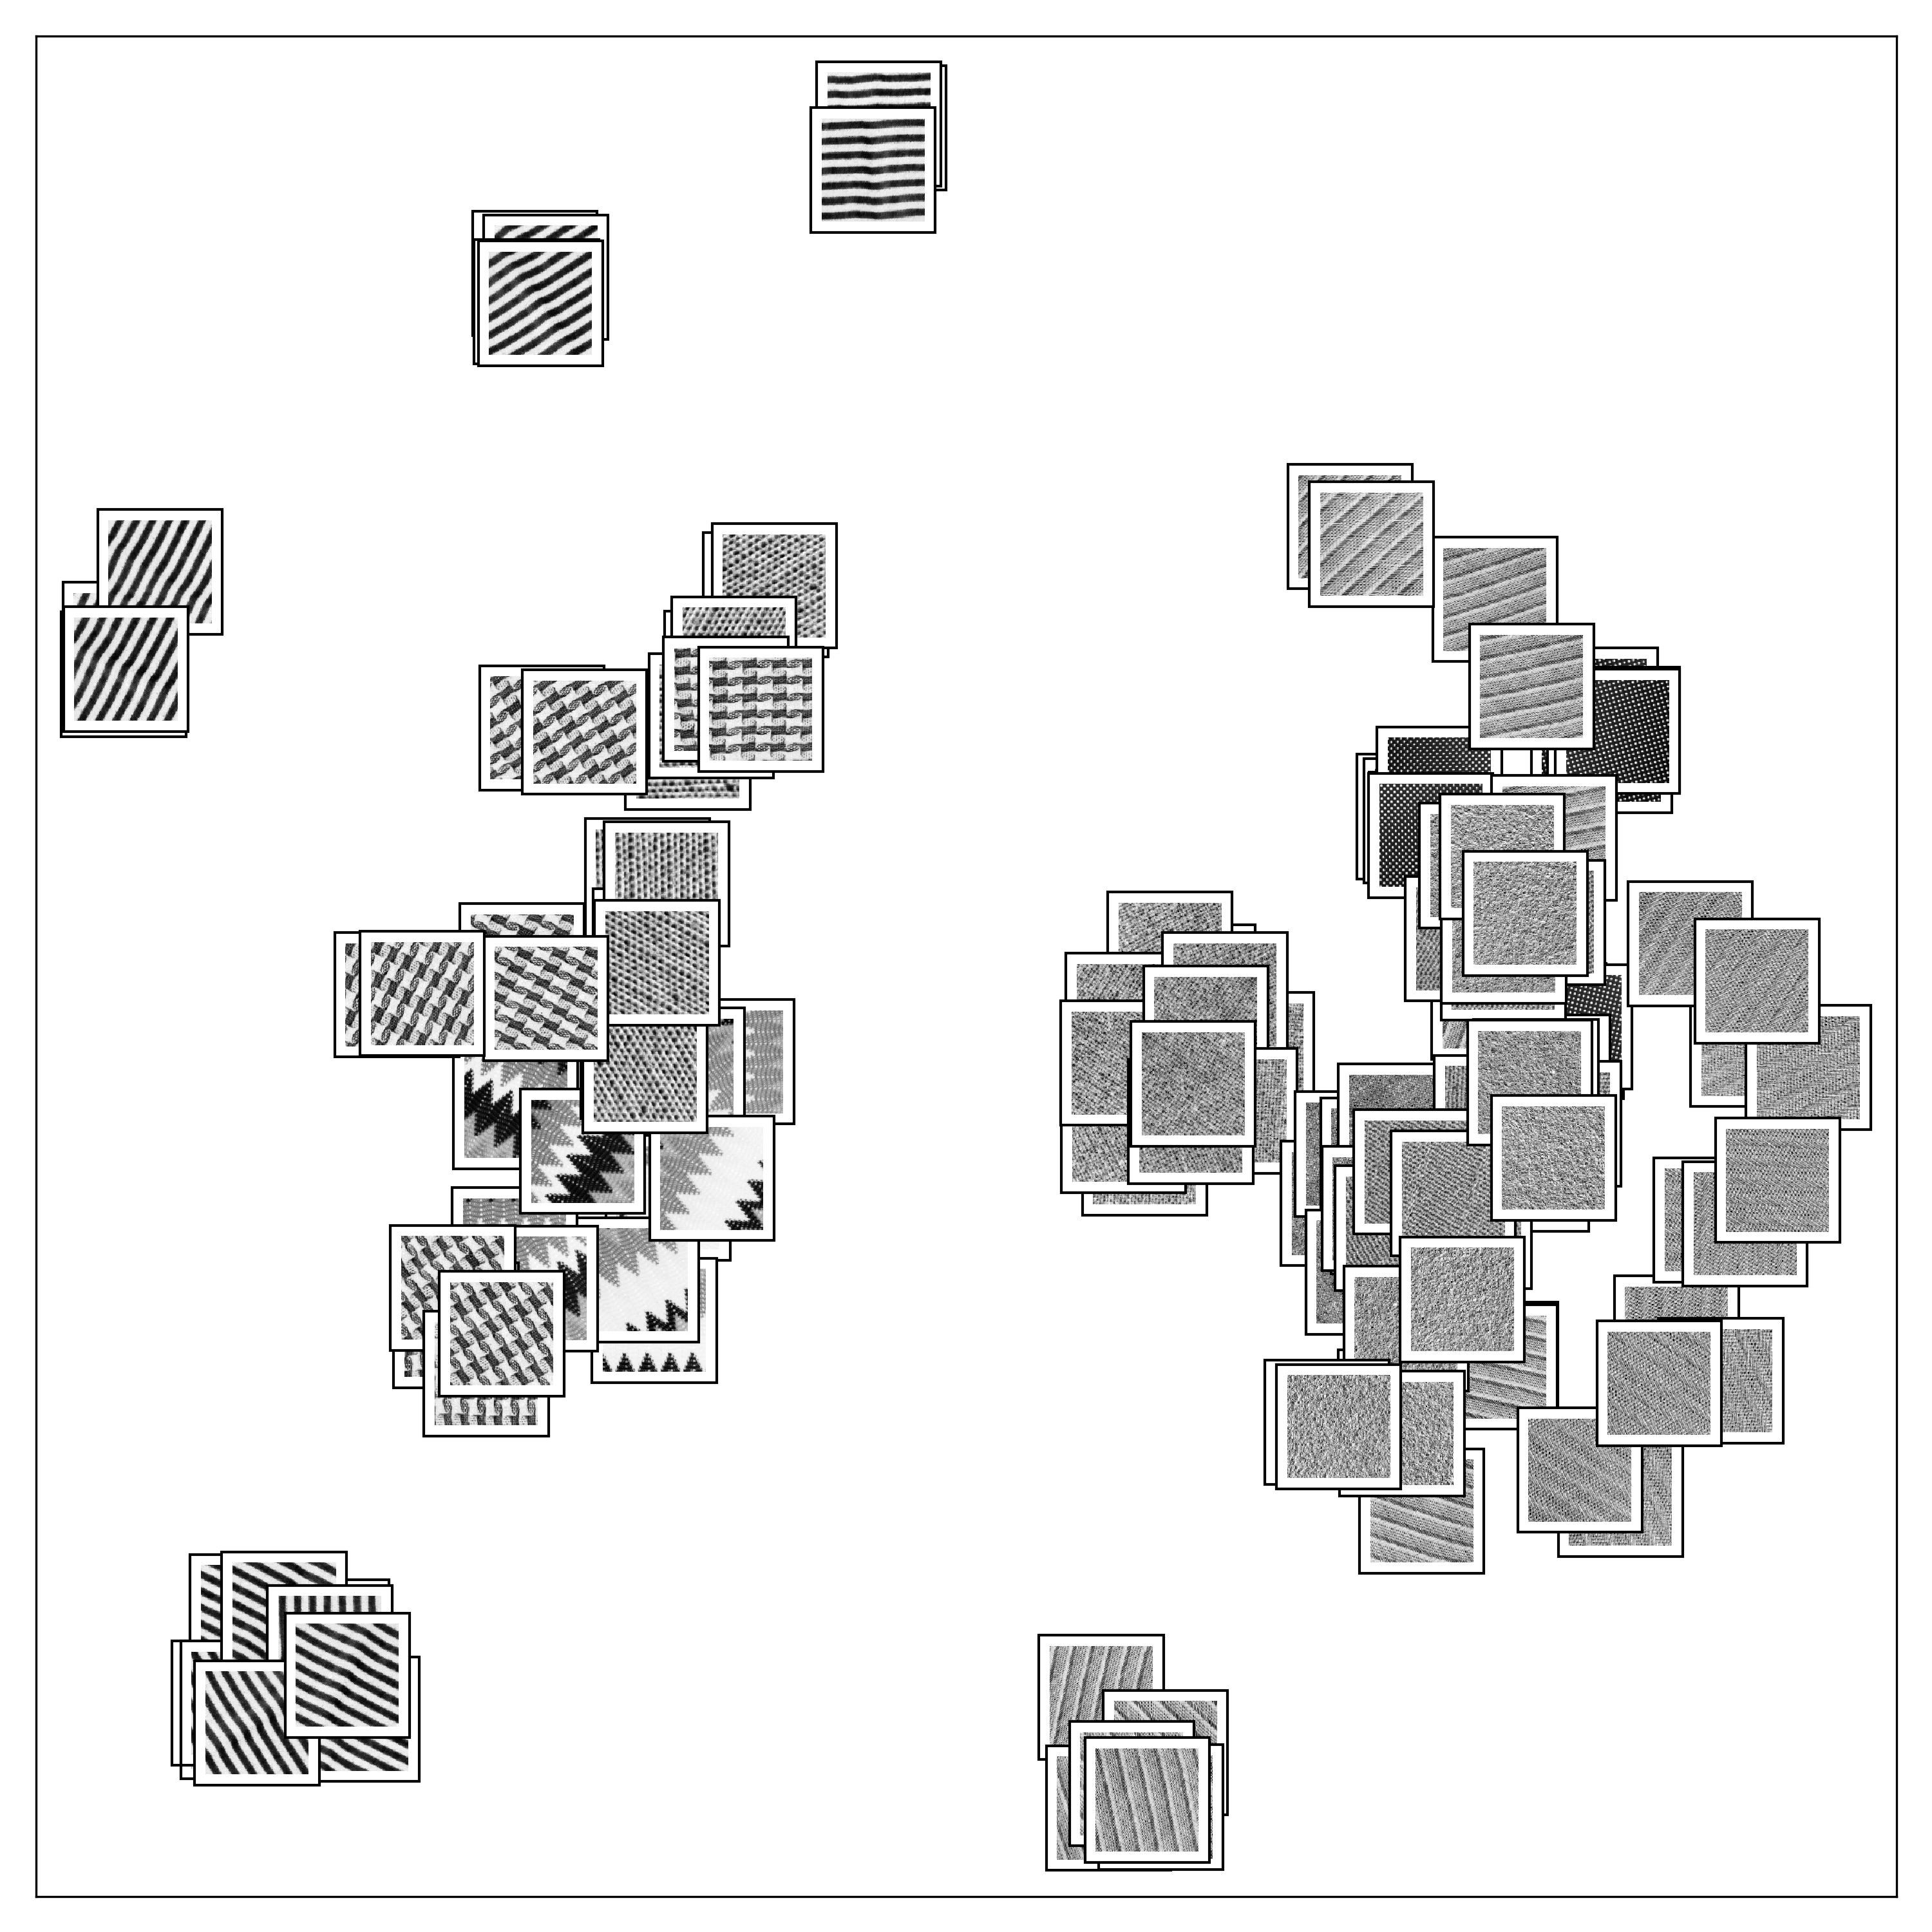
\includegraphics[width=0.7\textwidth]{MDS_Inter}
 \caption{MDS texture projection using the histogram intersection}
 \label{fig:MDS_Inter} 
\end{figure}

\begin{figure}[!ht]
 \centering    
 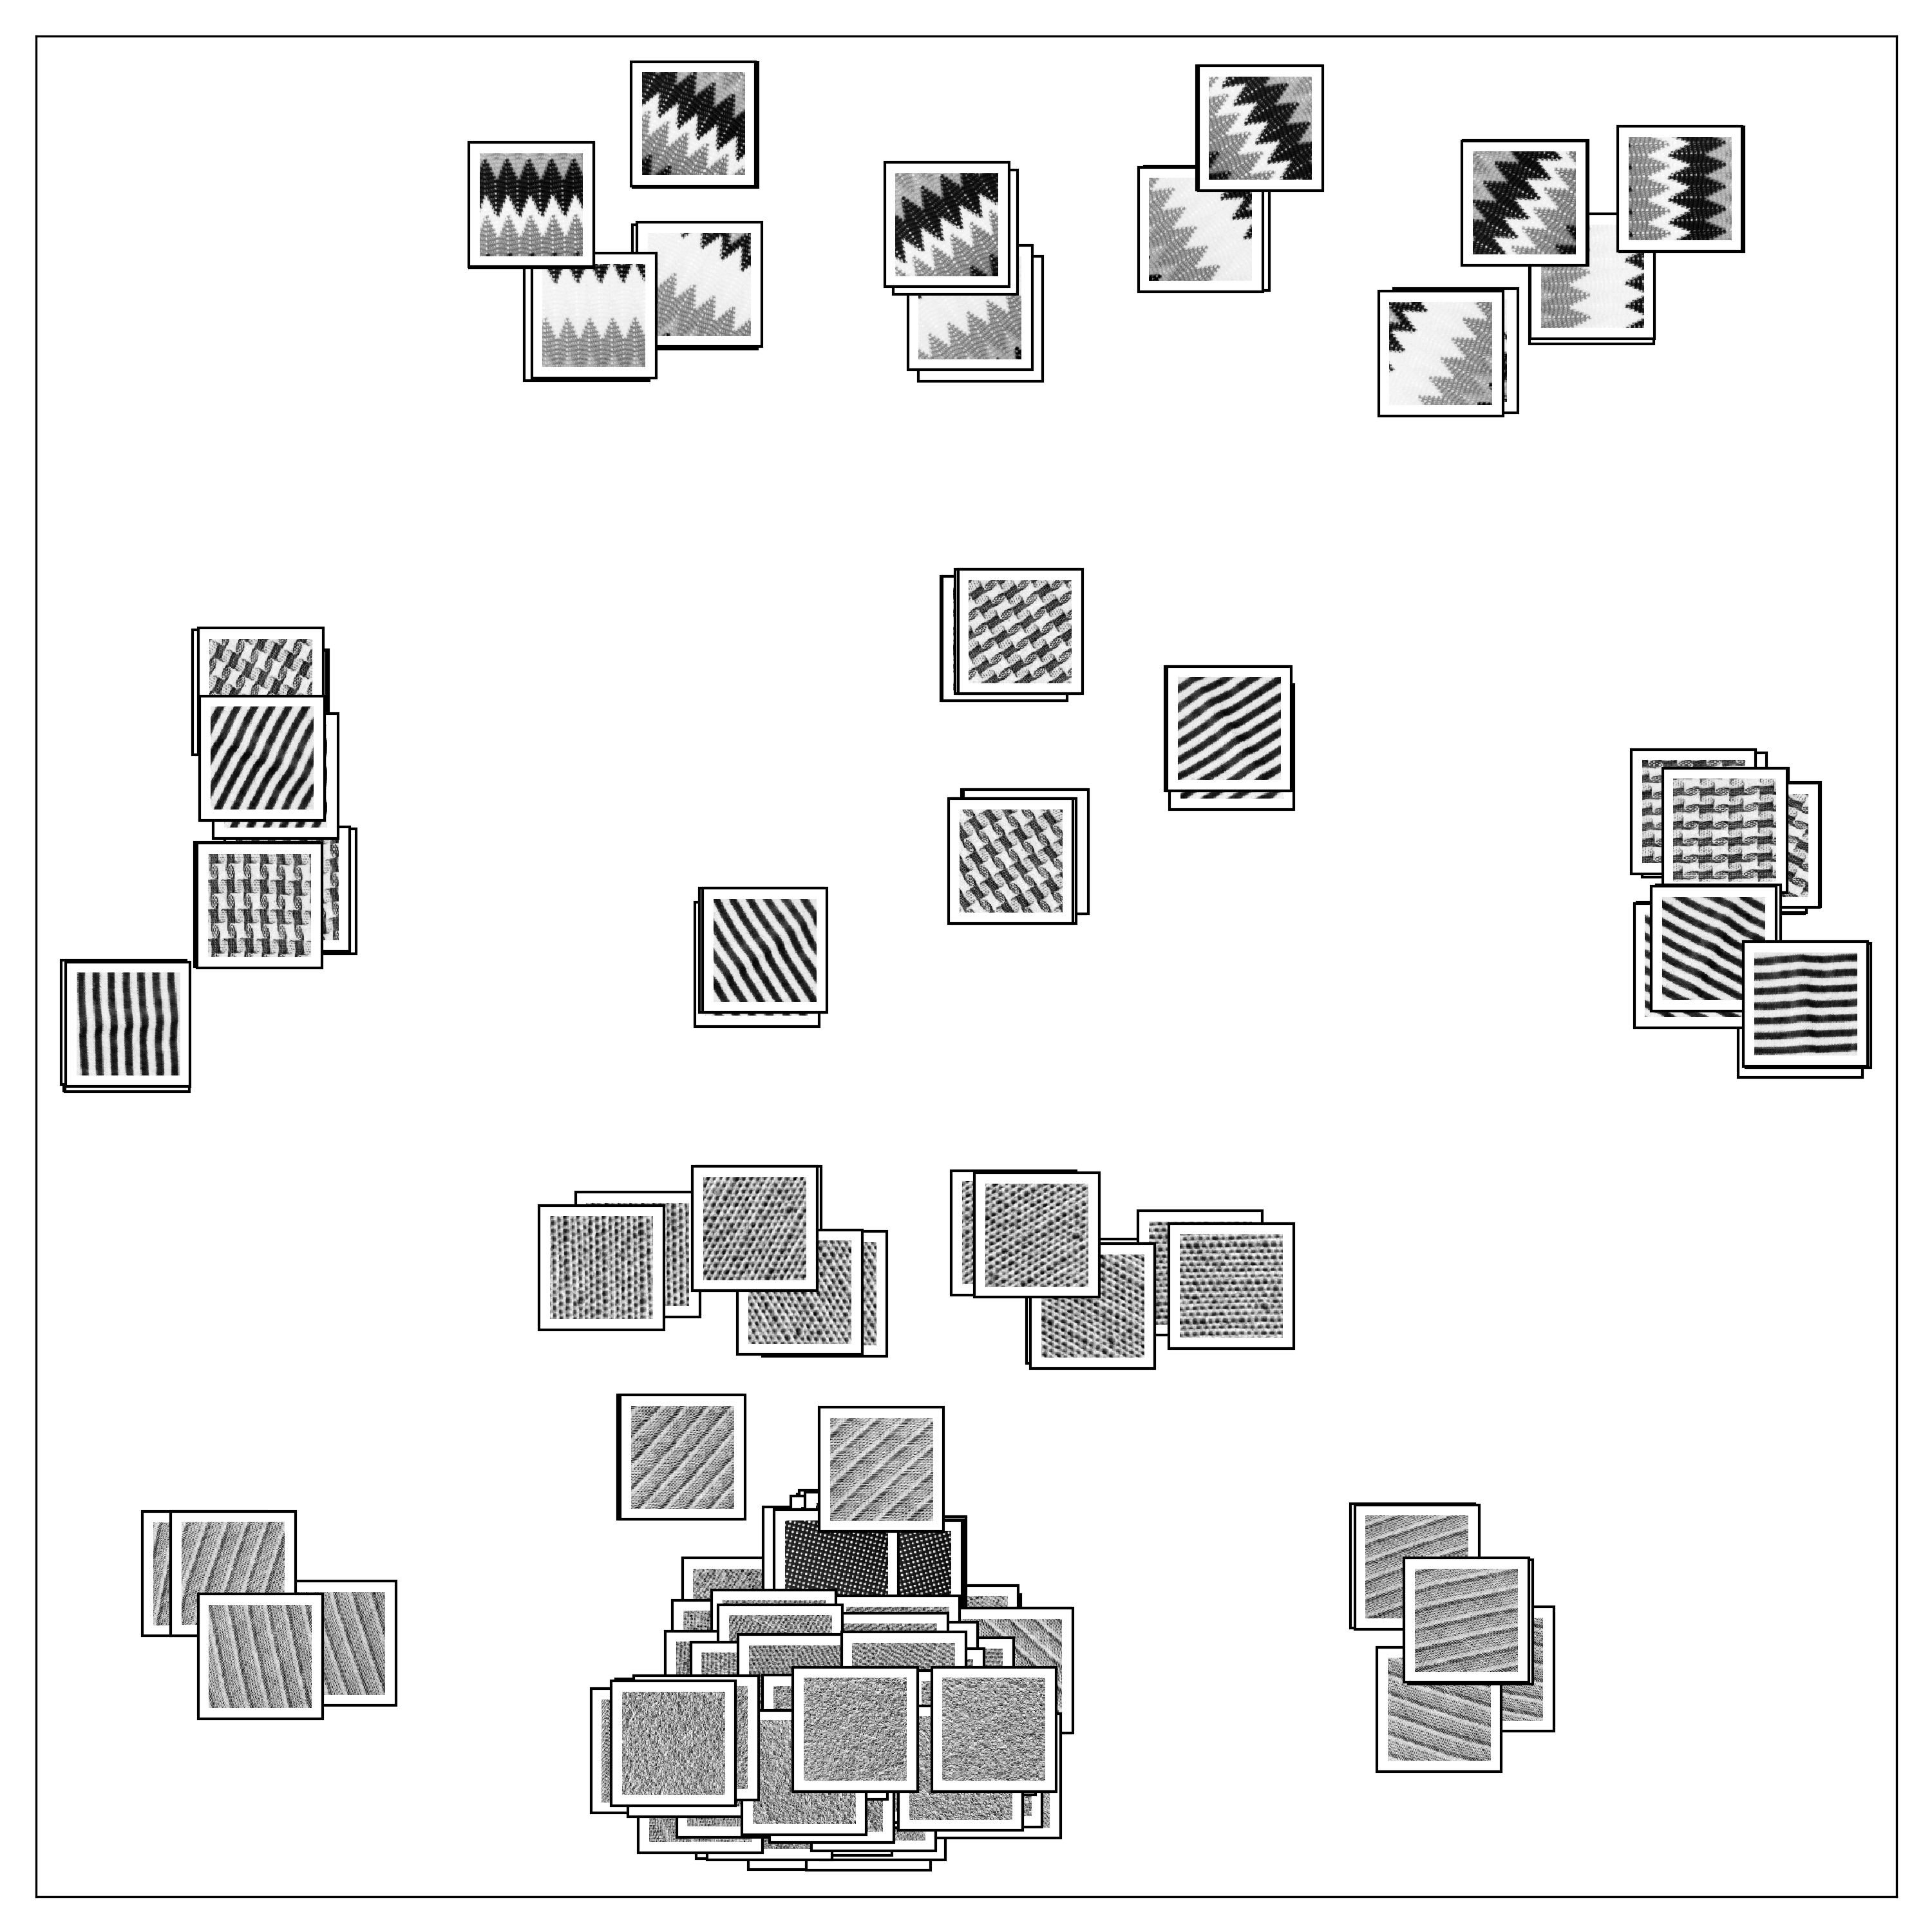
\includegraphics[width=0.7\textwidth]{MDS_Corr}
 \caption{MDS texture projection using the histogram correlation}
 \label{fig:MDS_Corr} 
\end{figure}

\begin{figure}[!ht]
 \centering    
 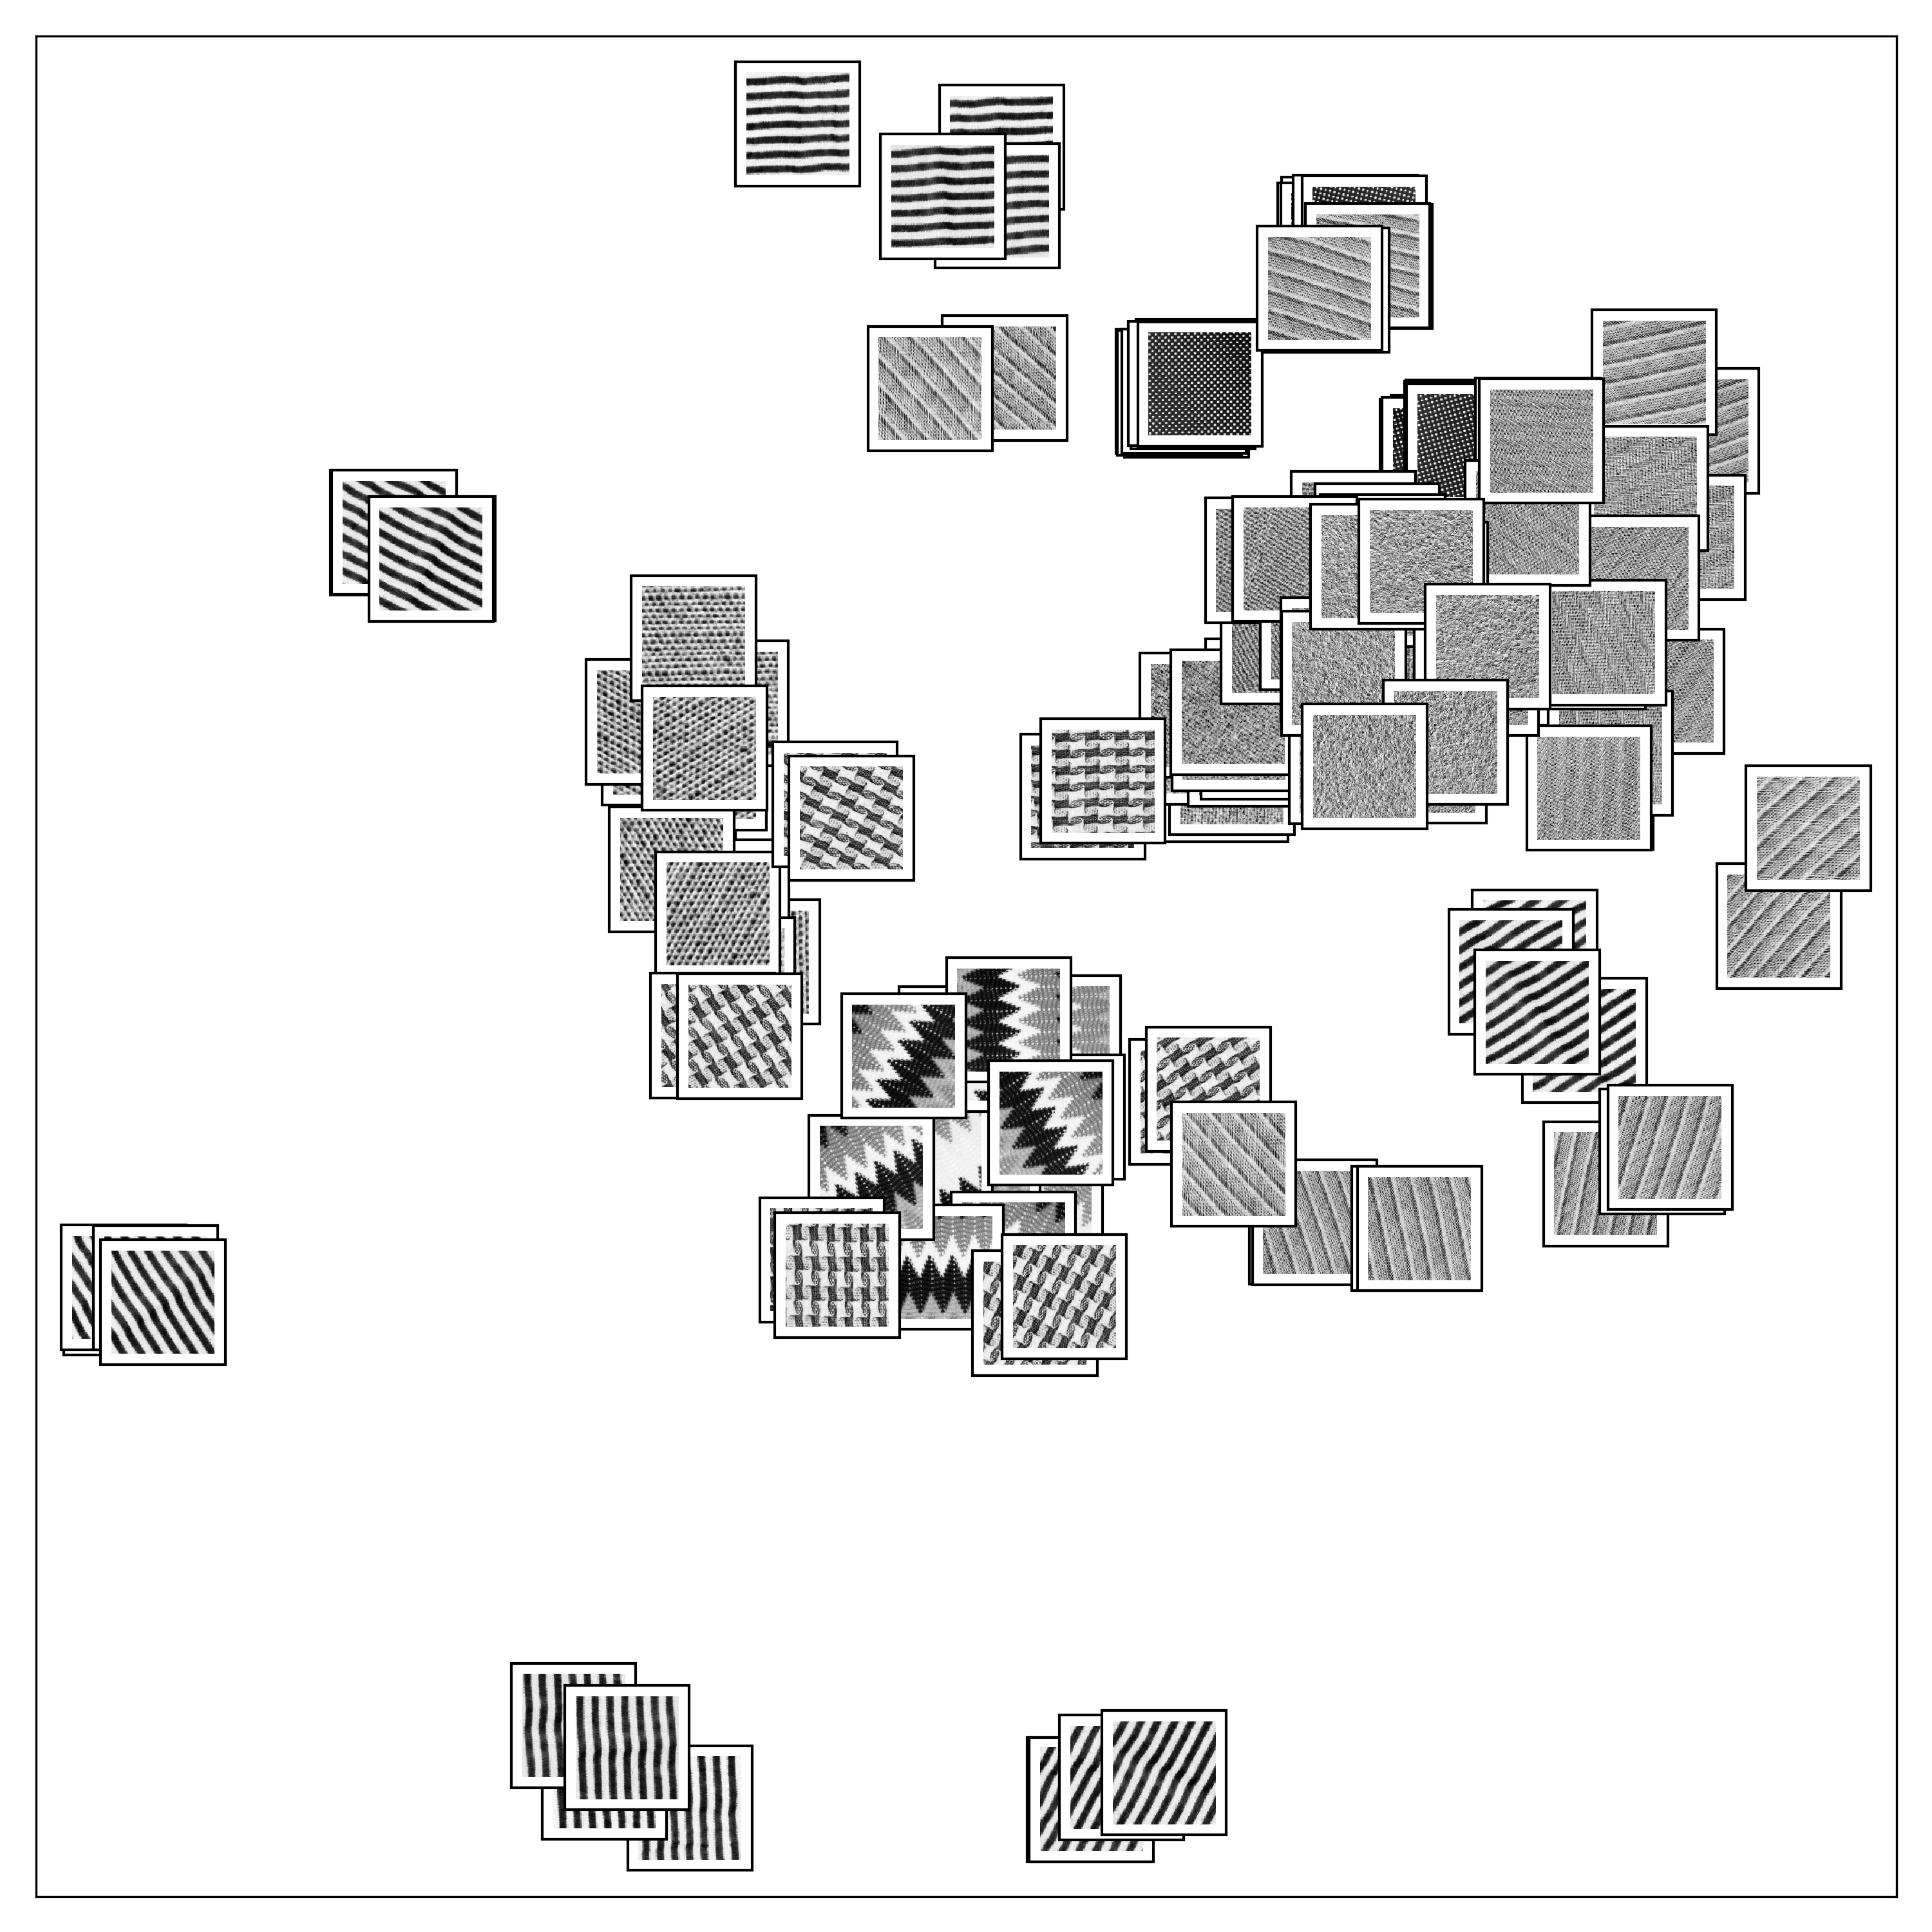
\includegraphics[width=0.7\textwidth]{MDS_Chi2}
 \caption{MDS texture projection using the $\chi^2$ statistic}
 \label{fig:MDS_Chi2} 
\end{figure}

\begin{figure}[!ht]
 \centering    
 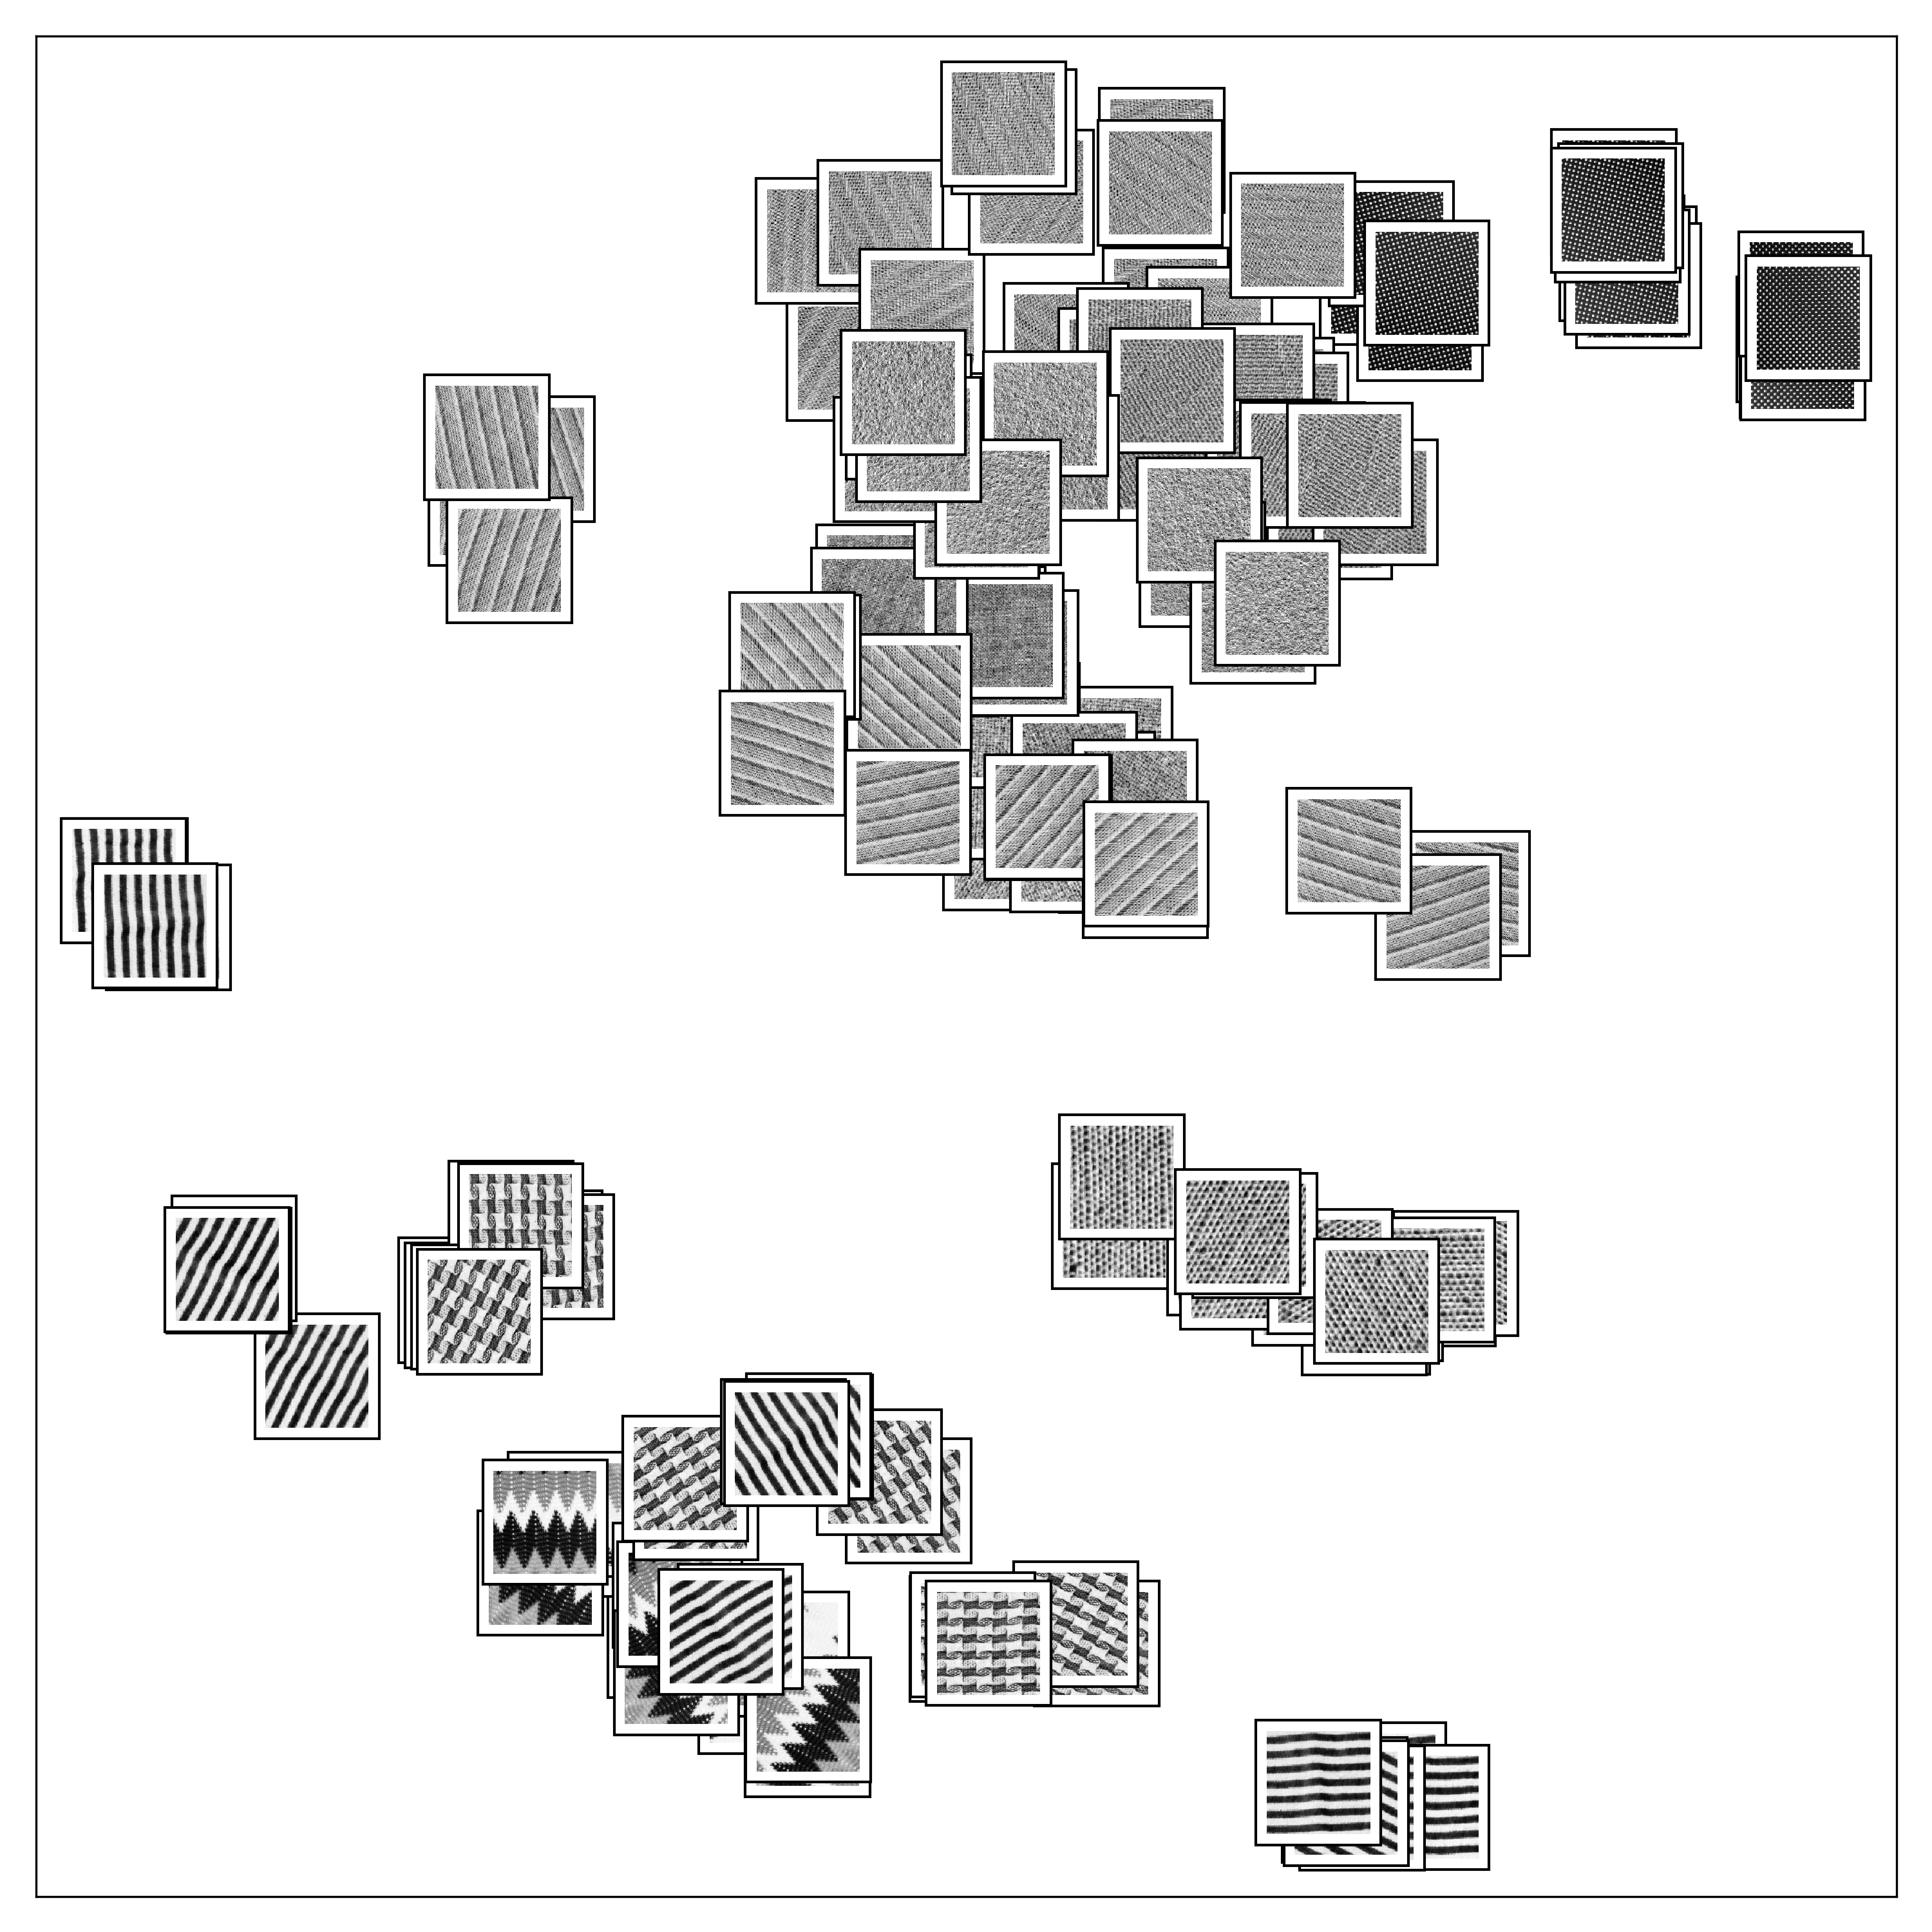
\includegraphics[width=0.7\textwidth]{MDS_Bhatt}
 \caption{MDS texture projection using the Bhattacharyya distance}
 \label{fig:MDS_Bhatt} 
\end{figure}

\begin{figure}[!ht]
 \centering    
 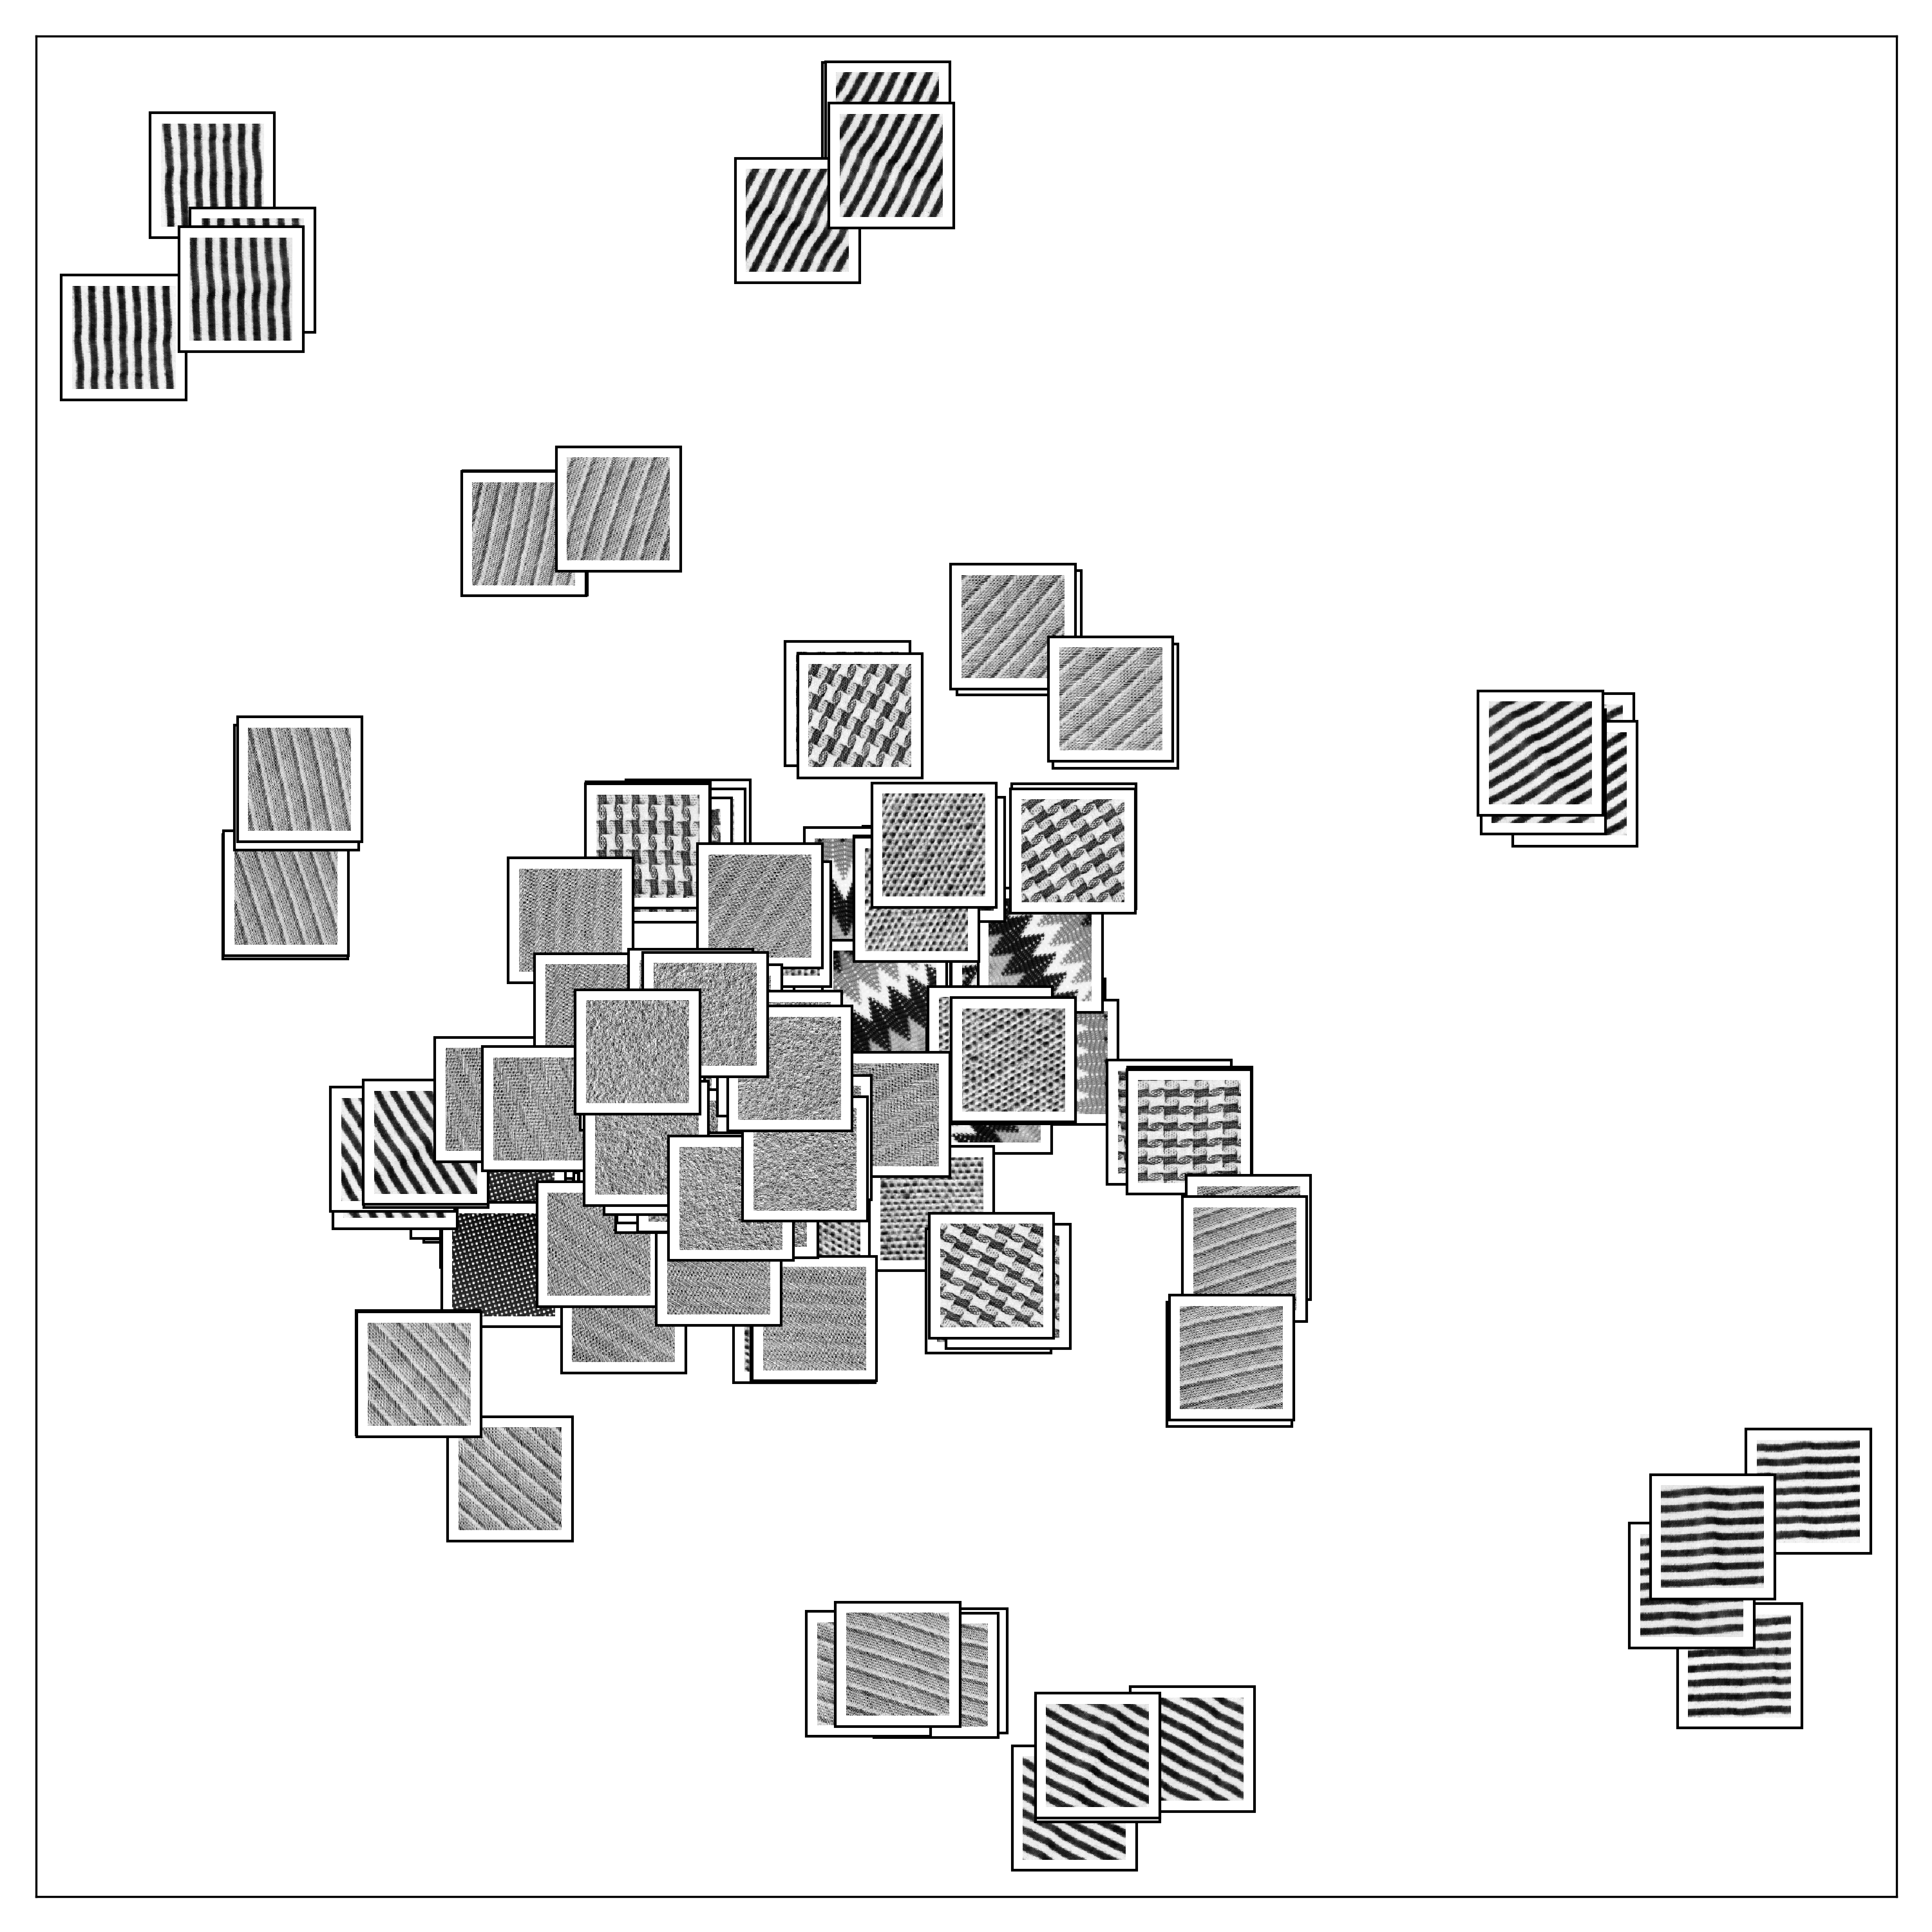
\includegraphics[width=0.7\textwidth]{MDS_KL}
 \caption{MDS texture projection using the Kullback-Leibler divergence}
 \label{fig:MDS_KL} 
\end{figure}

\begin{figure}[!ht]
 \centering    
 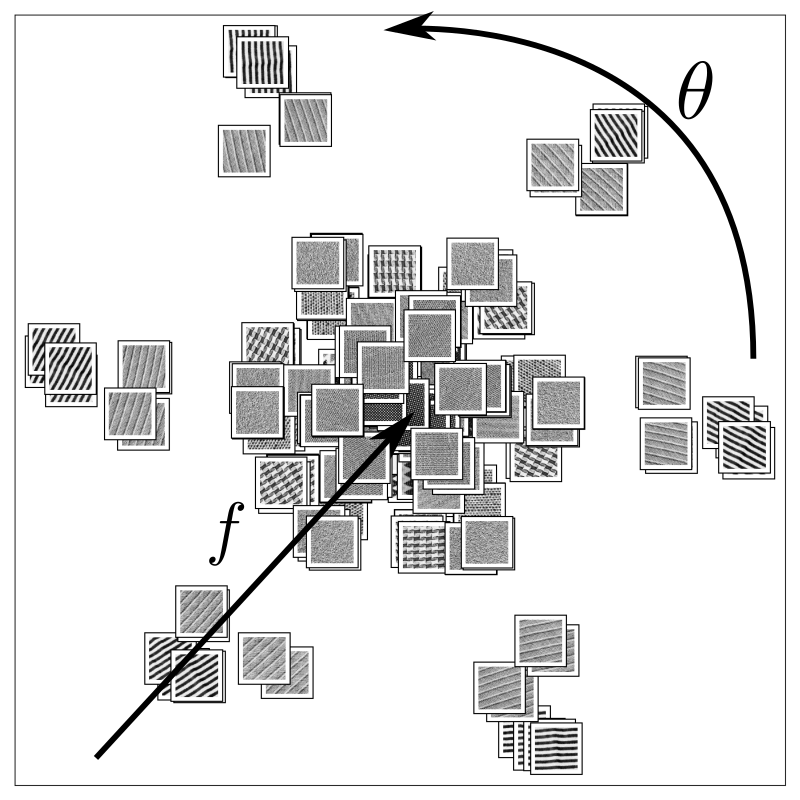
\includegraphics[width=0.7\textwidth]{MDS_EMD2}
 \caption{MDS texture projection using the Earth Mover's Distance}
 \label{fig:MDS_EMD} 
\end{figure}